
\section{Pull-back Prior}\label{sec:pull_back_prior}

\subsection{Intuition of Pull-back Prior}\label{subsec:intuition}

The formula of Pull-back Prior is given by:
\begin{equation}\label{eq:pull_back_prior}
	p_\lambda(z) = \frac{1}{Z} p_\mathcal{N}(z) * e^{- \beta * D(G(z))} \tag{4}
\end{equation}
where $p_\mathcal{N}$ is a simple prior, $D$ is a discriminator, $G$ is the generator $G(z) = \E_{p_\theta(x|z)} x$, $Z$ is the partition function $Z = \int_{\mathcal{Z}} p_\mathcal{N}(z) \exp\{- \beta * D(G(z))\} \dd z$ and $\beta$ is a learnable scalar.

An intuitive explanation of Pull-back Prior is given following: We would like to get a more powerful prior than simple prior $p_\mathcal{N}$. A simple way is to improve the density of $z$ which generates better data and decrease the density of $z$ which generates worse data. $D$ is a discriminator to assess the quality of $x$. When $D(x)$ is less, $x$ is more similar to real data and of higher quality, as shown in \cref{fig:interpolate}. We could pull-back the discriminator from data space to latent space, and function $D(G(z))$ represents the quality of the data generated by $z$. To improve and decrease the density at better $z$ and worse $z$, we modify $p_\mathcal{N}(z)$ by $\beta * D(G(z))$ and then normalize it by $Z$, and finally we obtain the Pull-back Prior. 

We obtain the basic formula of Pull-back Prior, and $p_\mathcal{N}$ is a special case $\beta = 0$. The theoretical derivation for Pull-back Prior is provided in \cref{subsec:inference}. However, it remains some troubles about how to determine $\beta$, calculate $Z$ and select $D$. 

\begin{figure}[tb]
	\centering
	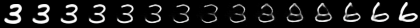
\includegraphics[width=0.9\columnwidth]{../figures/interpolate}
	\caption{
	The discriminators on above images (generated by linear interpolation of two sample from $q_\phi(z)$), are better at both sides and worse at mid, which validates the intuition that discriminator can assess the quality of images. Moreover, the density of $z$ which generate better images will increase, and the density of $z$ which generate worse images will decrease. 
%2825-plot_samples mean and std is 9.528099, 0.0050279954
%[array([[9.547822]], dtype=float32), array([[9.583102]], dtype=float32), array([[9.603901]], dtype=float32), array([[9.626318]], dtype=float32), array([[9.633714]], dtype=float32), array([[9.632847]], dtype=float32), array([[9.631333]], dtype=float32), array([[9.640044]], dtype=float32), array([[9.631817]], dtype=float32), array([[9.654361]], dtype=float32), array([[9.641564]], dtype=float32), array([[9.600273]], dtype=float32), array([[9.559095]], dtype=float32), array([[9.533435]], dtype=float32), array([[9.468535]], dtype=float32)]
%Normalized is [  3.92263684,  10.93934971,  15.07598834,  19.53442519,
%        21.00538915,  20.83295462,  20.53184058,  22.26434018,
%        20.62810161,  25.11179704,  22.56664754,  14.35442841,
%         6.16468344,   1.06125793, -11.84647066]
	}
	\label{fig:interpolate}
\end{figure}

\subsection{How to determine $\beta$}\label{subsec:determine_beta}

$\beta$ in \cref{eq:pull_back_prior} represents how far $p_\lambda$ is from $p_\mathcal{N}$, but how to decide the value of $\beta$? When $\beta$ is smaller, the difference between $p_\lambda$ and $p_\mathcal{N}$ is less, \IE the influence of discriminator is severely limited. When $\beta$ is larger, $p_\lambda$ is farther from $p_\mathcal{N}$. Noticing that in \cref{eq:final_optimization}, we simplify the optimization of $D$ by an approximated $D$, if $p_\lambda$ is too far from $p_\mathcal{N}$, this approximation will become invalid. Consequently, $\beta$ should be set to an appropriate value which can't severely limit the influence of discriminator and could ensure that approximated $D$ is valid. It is important to realize that the Pull-back Prior is serving for better ELBO. Whatever the function family of $p_\lambda$ is limited or approximation $D$ is invalid, the ELBO will suffer. Therefore, it is reasonable to search $\beta$ by the optimization for ELBO ($\lambda$ contains $\beta$ and $\omega$, which is the parameters of $D$):
\begin{equation}
	\beta = \arg \min_{\beta} \mathcal{L}(\theta, \phi, \lambda) = \arg \min_{\beta} \mathcal{L}(\theta, \phi, \beta, \omega) \tag{5}
\end{equation}
The optimization process of $\beta$ depends on $\partial \mathcal{L}/\partial \beta$:
\begin{align*}\label{eq:behavior_of_beta}
\frac{\partial \mathcal{L}}{\partial \beta} &= \E_{q_\phi(z)}[ -D(G(z))] - \frac{\partial Z}{\partial \beta} \\
&= \E_{p_\lambda(z)}[ D(G(z))] - \E_{q_\phi(z)}[ D(G(z))]  \tag{6}
\end{align*}
The 1st term in \cref{eq:behavior_of_beta} is the mean of discriminator on data generated from $p_\lambda$. The 2nd term in \cref{eq:behavior_of_beta} is the mean of discriminator on reconstructed data which is nearly same as real data when reconstruction is well-trained. Hence, $\partial \mathcal{L}/\partial \beta = 0$ represents that the discriminator can't distinguish the reconstructed data (nearly same as real data) and generated data. It coincides the philosophy of GAN.

\subsection{How to calculate $Z$}\label{subsec:determine_z}

We have known that $Z = \int_{\mathcal{Z}} p_\mathcal{N}(z) \exp\{- \beta * D(G(z))\} \dd z$, denoted by $\int_{\mathcal{Z}} f_\lambda(z) \dd z$. It is natural to determine $Z$ by importance sampling $Z = \E_{p_\mathcal{N}(z)} \exp\{- \beta * D(G(z))\}$ as ~\cite{bauer2019resampled} did. By the theory of importance sampling, the variance of the estimation of $Z$ is $Var_{p_b}[\frac{f_\lambda}{p_b}]$, where $p_b$ is another distribution. Hence, the variance is smallest when $p_b = p_\lambda$ and it is larger when $p_\lambda$ is farther from $p_b$. If we choose $p_b$ as $p_\mathcal{N}$, when $\beta$ is large, the variance will be large and it will influence the optimization and evaluation. 

The optimal choice for $p_b$ is $p_\lambda$ itself but it is hard to sample from $p_\lambda$ during training. We try to find a distribution which is near to $p_\lambda$ and easy-sampling. As \cref{eq:behavior_of_beta} shows, when $\beta$ approaches optimal, the discriminator can't distinguish the data generated by $p_\lambda(z)$ and $q_\phi(z)$.  \cref{eq:second-decomposition} also shows that when $p_\lambda(z)$ is optimized for $\mathcal{L}(\theta, \phi, \lambda)$, it approaches to $q_\phi$. Consequently, it is reasonable to choose $q_\phi$ as $p_b$. 

However, as we mentioned before, $q_\phi(z)$ is intractable to compute the exact density. We introduce a bias estimation for $q_\phi(z)$, which will lead to the bias estimation for $Z$. 
\begin{equation*}
	q_\phi(z) = \E_{p^*(x)} q_\phi(z|x) \approx \frac{1}{N}\sum_{i=1}^N q_\phi(z|x^{(i)}) \geq \frac{1}{N} q_\phi(z|x^{(j)})
\end{equation*}
where $x^{(j)}$ is one of real data, $N$ is the size of training set. To reduce the error, $q_\phi(z|x^{(j)})$ should be one of the largest in summation. Therefore, we firstly choose $x^{(j)}$, then sample $z$ from $q_\phi(z|x^{(j)})$ (by this way, $q_\phi(z|x^{(j)})$ will be large enough), and finally set $\frac{1}{N} q_\phi(z|x^{(j)})$ as a bias estimation for $q_\phi(z)$. When $p^*(x)$ consists of numerous data (\EG in MNIST the input of model is sampled from real images), $p^*(x)$ is sampled from another distribution $p^*(e)$, and $N$ might be very large. The situation with finite $N$ can be seen as a special case that $p^*(x|e) = \delta(x - e)$, so we could use signs $x, e$ on all datasets. We introduce another ELBO which use $q_\phi(z|e)$ instead of $q_\phi(z|x)$:
\begin{align*}~\label{eq:another_elbo}
	&\E_{p^*(x)} \ln p_\theta(x) \geq \E_{p^*(e)} \E_{p^*(x|e)} \ln \E_{q_\phi(z|e)} \frac{p_\theta(x|z)p_\theta(z)}{q_\phi(z|e)} \\
	 &= \E_{p^*(e)} \E_{p^*(x|e)} \E_{q_\phi(z|e)} \ln \frac{p_\theta(x|z)p_\theta(z)}{q_\phi(z|e)} \tag{7} \\
	 &= \E_{p^*(x)} \ln p^*(x) - \E_{p^*(e)} \E_{p^*(x|e)} KL(q_\phi(z|e), p_\theta(z|x))
\end{align*} 
where $p^*(x|e)$ means the sampling process from $e$, usually Bernouli distribution. \cref{eq:another_elbo} is similar to the original ELBO~\cref{eq:ELBO}, and the above conclusion about learnable prior holds for \cref{eq:another_elbo} by repeating above inference. % Additionally, when $p_\theta(x|z)$ and $p^*(x|e)$ is both Bernouli, term $\E_{p^*(x|e)} \ln p_\theta(x|z)$ has analytical solution $x\log e+(1-x)\log(1-e)$, which could make the training and evaluation more stable (don't need sample $x$). 
Since $q_\phi(z|e)$ is known, above bias estimation of $q_\phi(z)$ is feasible by $\frac{1}{N} q_\phi(z|e^{(j)})$. $\hat{q}_\phi(z)$ denotes the bias estimation of $q_\phi(z)$. Then, a bias estimation $\hat{Z}$ is given by:
\begin{align*}\label{eq:Z_estimator}
	Z = \E_{q_\phi(z)}\frac{f_\lambda(z)}{q_\phi(z)} \leq \E_{q_\phi(z)} \frac{f_\lambda(z)}{\hat{q}_\phi(z)} = \hat{Z} \tag{8}
\end{align*}

Because $\beta$ is optimized from small to large during training, we use both estimations for $Z$ in training. After training, $\beta$ is large and $p_\lambda$ approach to $q_\phi$ by \cref{eq:behavior_of_beta}, therefore we use \cref{eq:Z_estimator} for computing the final value of $Z$. The last thing we need to check is that the bias of estimation will not over-estimate the log-likelihood in evaluation:
\begin{equation*}
	p_\theta(x) = \E_{q_\phi(z|e)} \frac{f_\lambda(z) p_\theta(x|z)}{Z q_\phi(z|e)}  \geq \E_{q_\phi(z|e)} \frac{f_\lambda(z) p_\theta(x|z)}{\hat{Z} q_\phi(z|e)}
\end{equation*}
which means the estimation log-likelihood based on $\hat{Z}$ (RHS) is a lower bound of model density $p_\theta(x)$. 